\section{Model}\label{model}
\subsection{Delegates}
Figure \ref{Delegate} shows the number of delegates awarded after each primary/caucus per candidate. The results are displayed for each state until Super Tuesday. Biden is awarded with the most number number of delegates compared to other candidates. Buttigieg acquired the least number of delegates. 
\begin{figure}[H]
    \centering
    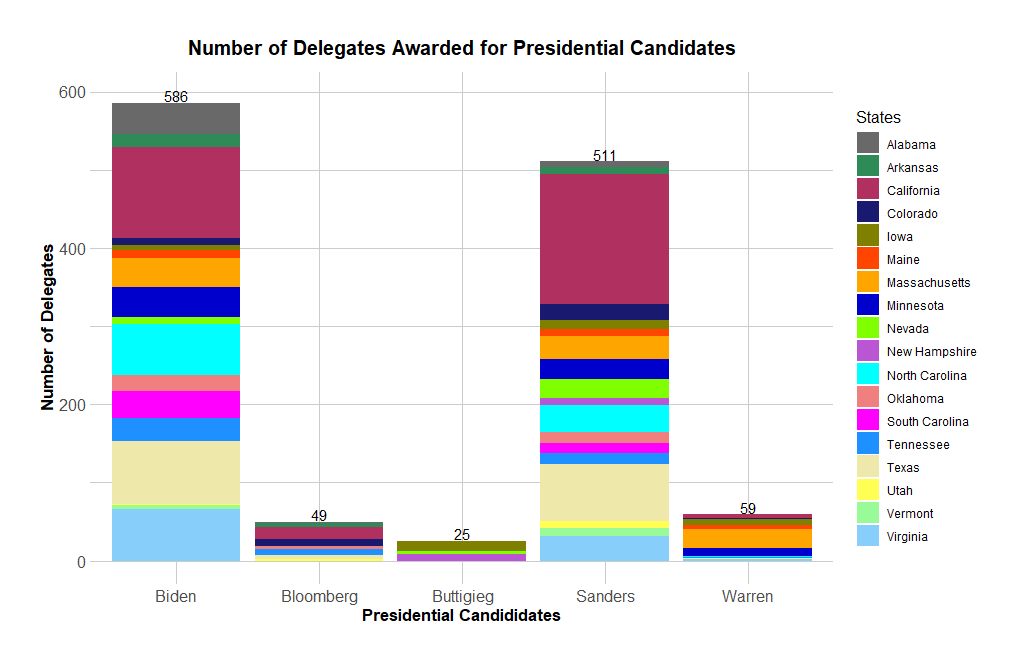
\includegraphics[width=0.9\textwidth]{figures/Delegate.png}
    \caption{Delegate}
    \label{Delegate}
\end{figure}

\subsection{Polling}
The poll data is collected and plotted for top five democratic candidates(Biden, Sanders, Warren, Bloomberg and Buttigieg). Data is plotted for both A rated and for all the polls as displayed in figures \ref{Updated-Polling-Data-1}, \ref{A-rated-polls} and \ref{All-rated-polls}. 
\begin{figure}[H]
    \centering
    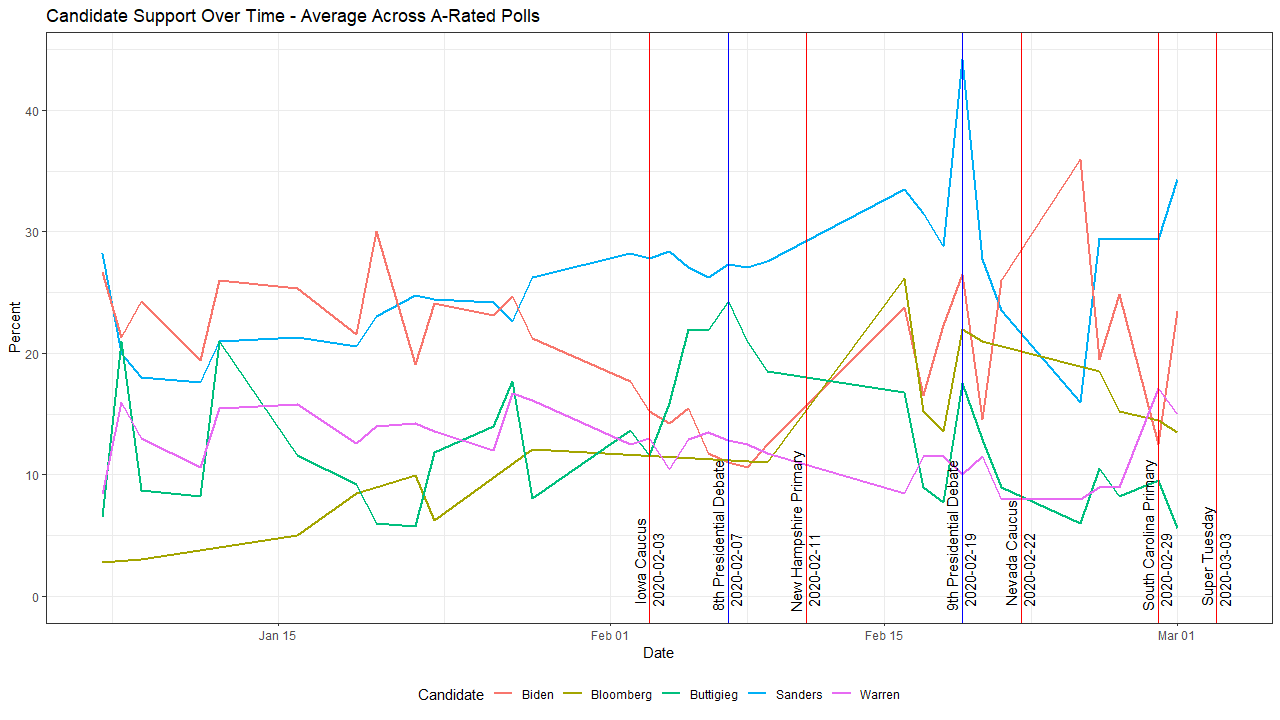
\includegraphics[width=0.9\textwidth]{figures/long-A-rated-polls.png}
    \caption{Updated Polling Data}
    \label{Updated-Polling-Data-1}
\end{figure}
Figure \ref{A-rated-polls} displays the support for candidates collected from A rated polls. At the end of  South Carolina Primary , it is observed that Sanders has the highest percentage of support is the highest and Buttigieg has the lowest percentage of support.  
\begin{figure}[H]
    \centering
    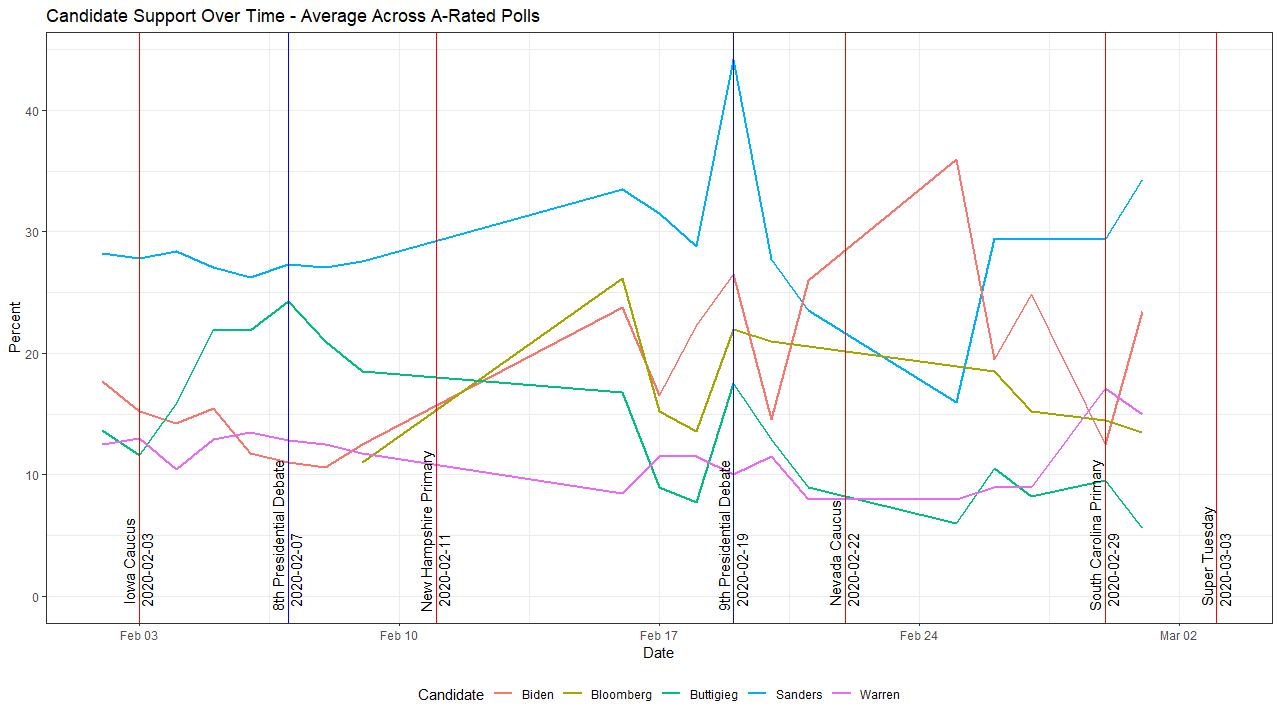
\includegraphics[width=0.9\textwidth]{figures/A-rated-polls.png}
    \caption{A Rated Polls}
    \label{A-rated-polls}
\end{figure}

Figure \ref{All-rated-polls} shows support for candidates until Super Tuesday from all rated polls. Biden's support shows a drop, making Biden the top candidate with highest percentage of support and Buttigieg with the lowest support percentage. 
\begin{figure}[H]
    \centering
    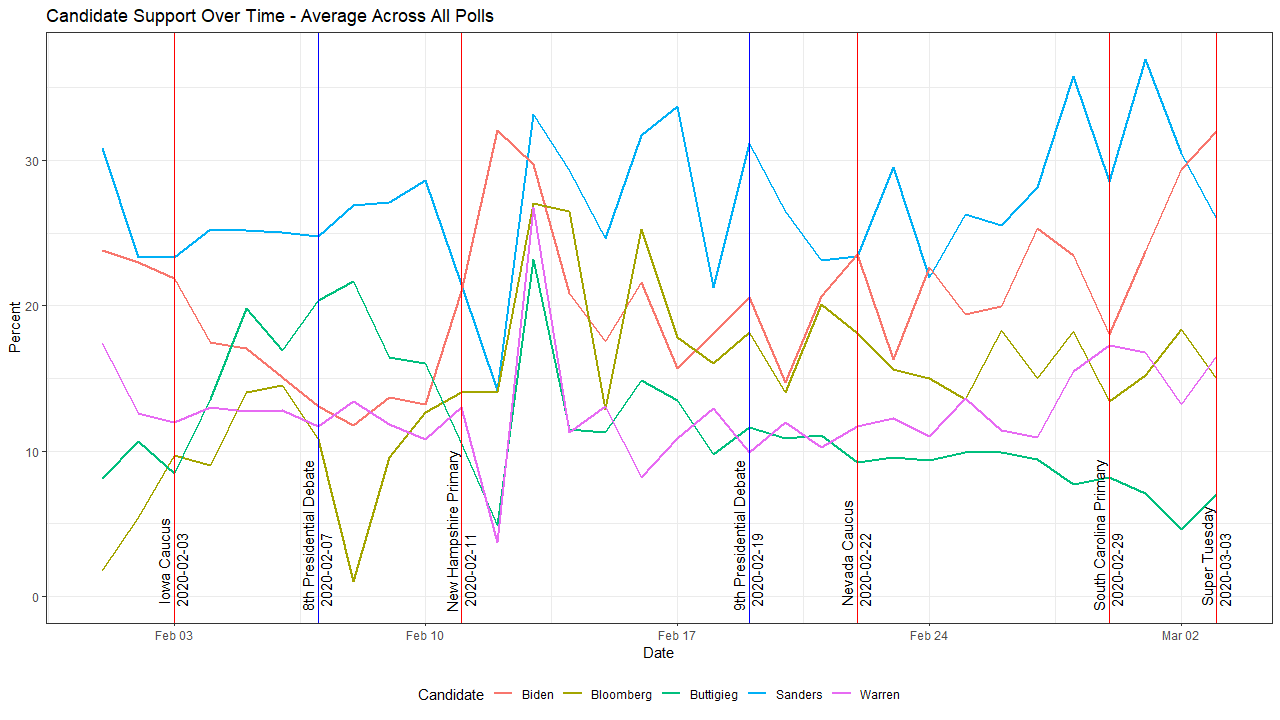
\includegraphics[width=0.9\textwidth]{figures/All-rated-polls.png}
    \caption{All Rated Polls}
    \label{All-rated-polls}
\end{figure}

Figure \ref{scatter-A-rated} shows support for candidates until South Carolina Primary. A slight drop is observed in Sanders' percentage of support after Nevada Caucus. Though there's a steady increase in Warren's support after Nevada caucus and South Carolina Primary, she still has the lowest percentage of support. 
\begin{figure}[H]
    \centering
    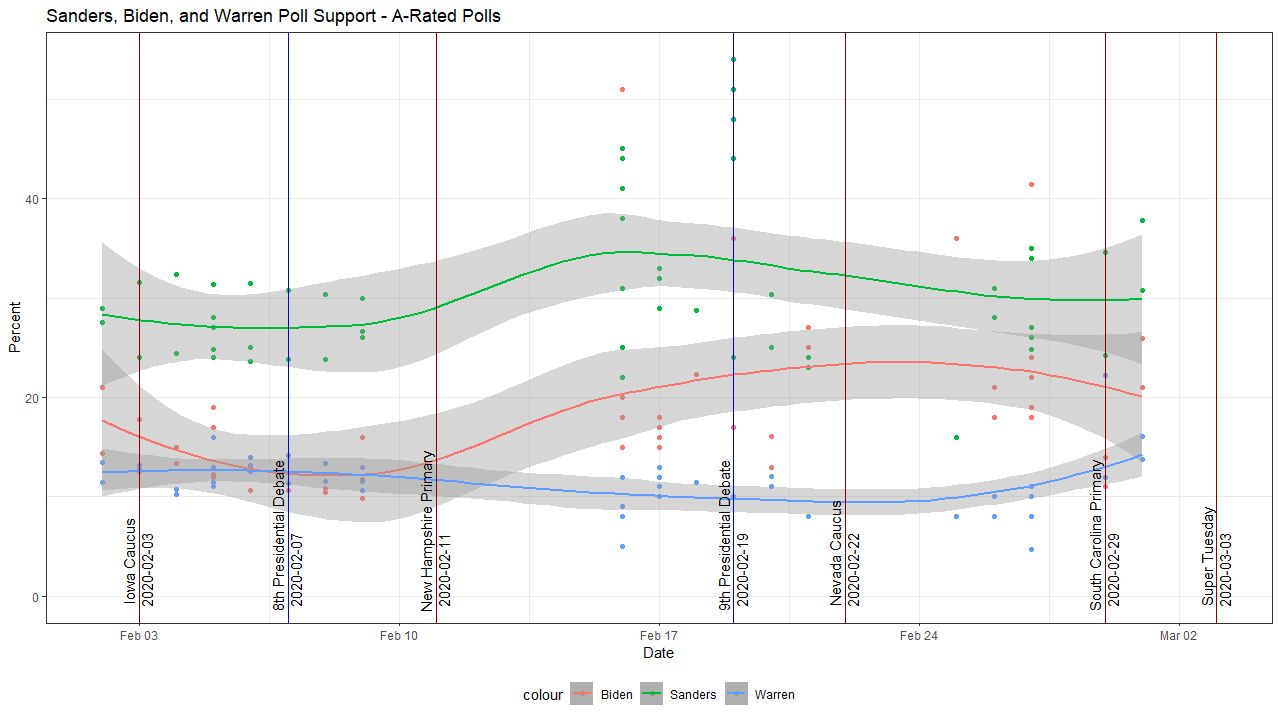
\includegraphics[width=0.9\textwidth]{figures/scatter-A-rated.png}
    \caption{Scatter Plot for A Rated Polls}
    \label{scatter-A-rated}
\end{figure}

Figure \ref{scatter-all} shows support for candidates until Super Tuesday. There is a steady increase in Sanders' percentage of support after South Carolina Primary. There is a sharp increase in Biden's percentage of support after South Carolina Primary,almost on par with Sanders. Warren's support has been consistently the lowest percentage of support compared to other candidates. 
\begin{figure}[H]
    \centering
    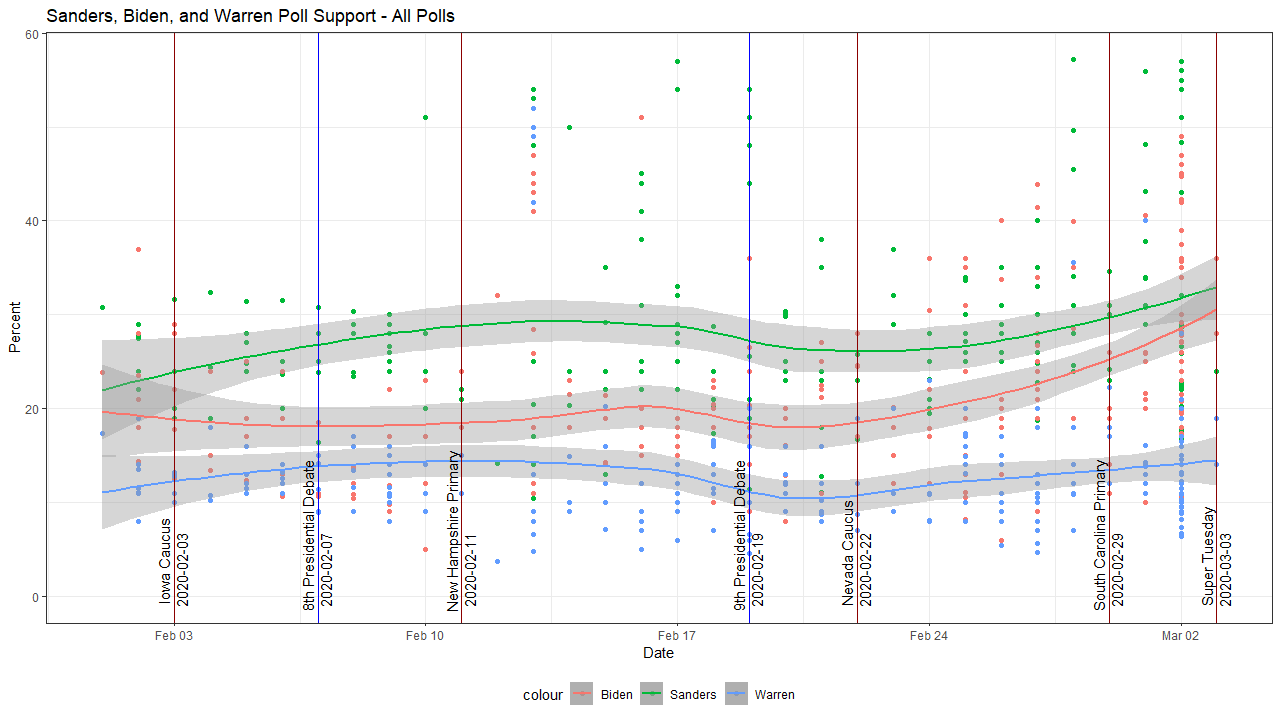
\includegraphics[width=0.9\textwidth]{figures/scatter-all.png}
    \caption{Scatter Plot for All Rated Polls}
    \label{scatter-all}
\end{figure}
Figure \ref{scatter-all-linear} shows the linear trend for candidate support until Super Tuesday. Overall, starting from Iowa Caucus to Super Tuesday, Sanders' support increases steadily whereas a progressive growth for support is observed in Biden's support percentage. Warren's support percentage shows a slight dip overtime.
\begin{figure}[H]
    \centering
    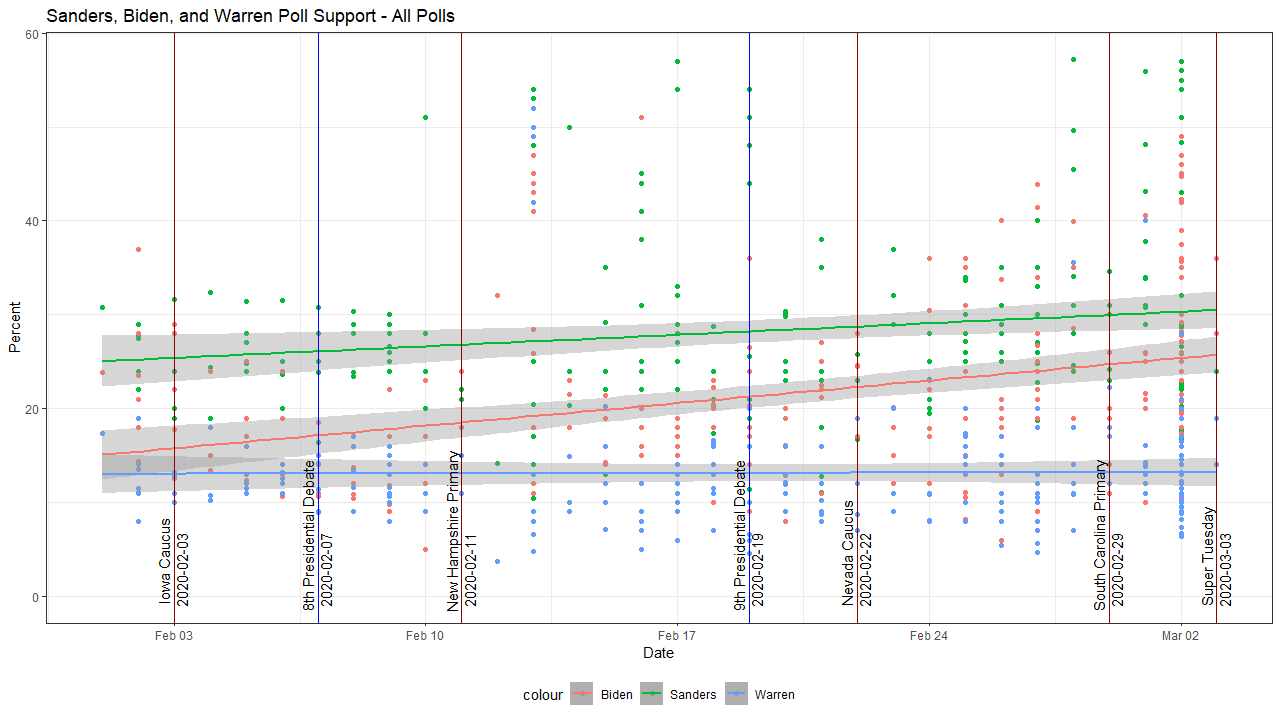
\includegraphics[width=0.8\textwidth]{figures/scatter-all-linear.png}
    \caption{Scatter Plot for All Rated Polls - Linear}
    \label{scatter-all-linear}
\end{figure}

\subsection{Spending}
Figures \ref{MoneyspendinAds} to \ref{Nevada} shows the amount of money spent on advertisements state wise(Iowa, New Hampshire and Nevada). 

\begin{figure}[H]
    \centering
    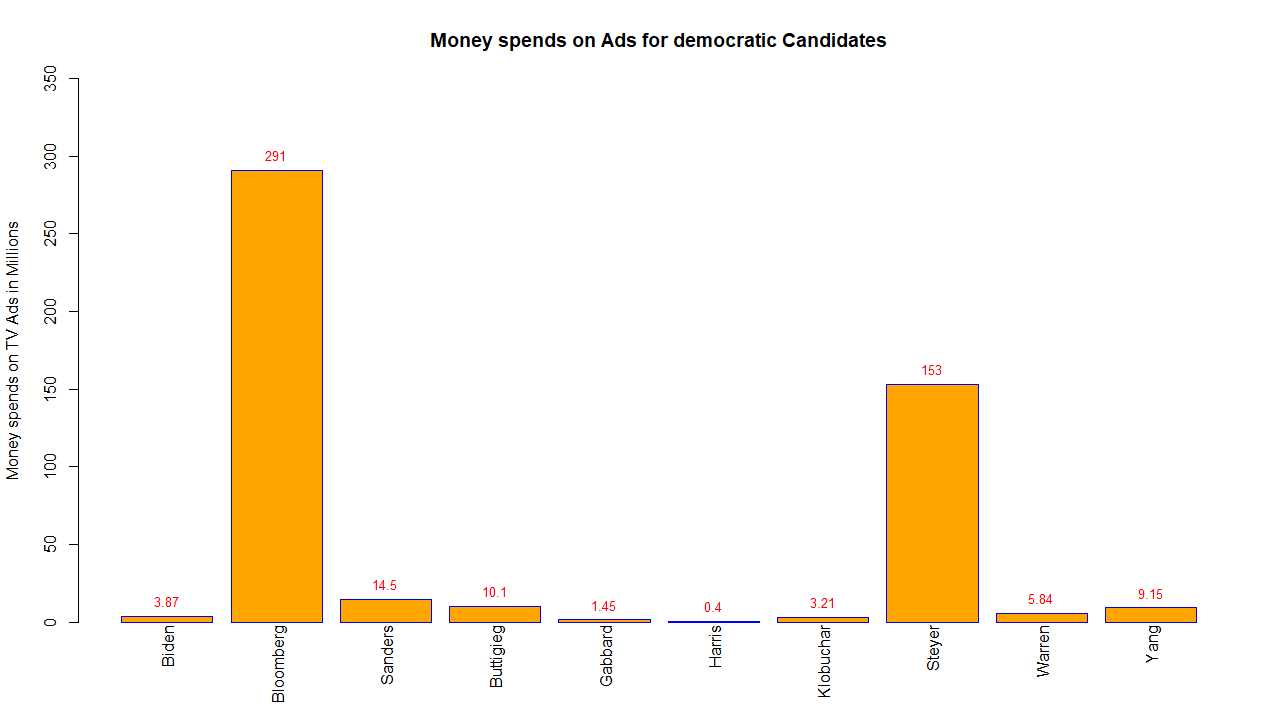
\includegraphics[width=0.9\textwidth]{figures/MoneyspendinAds.png}
    \caption{Money spending on Ads}
    \label{MoneyspendinAds}
\end{figure}

\begin{figure}[H]
    \centering
    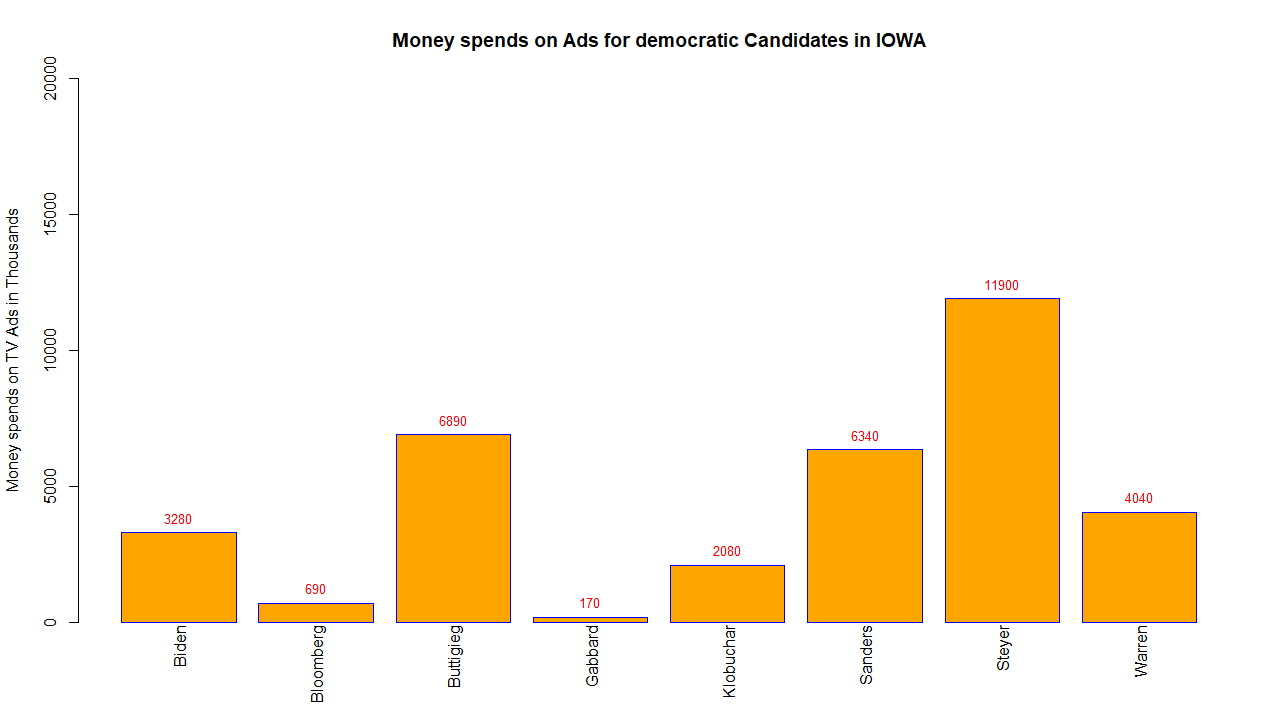
\includegraphics[width=0.9\textwidth]{figures/IOWA.png}
    \caption{Money spending on Ads in Iowa}
    \label{IOWA}
\end{figure}

\begin{figure}[H]
    \centering
    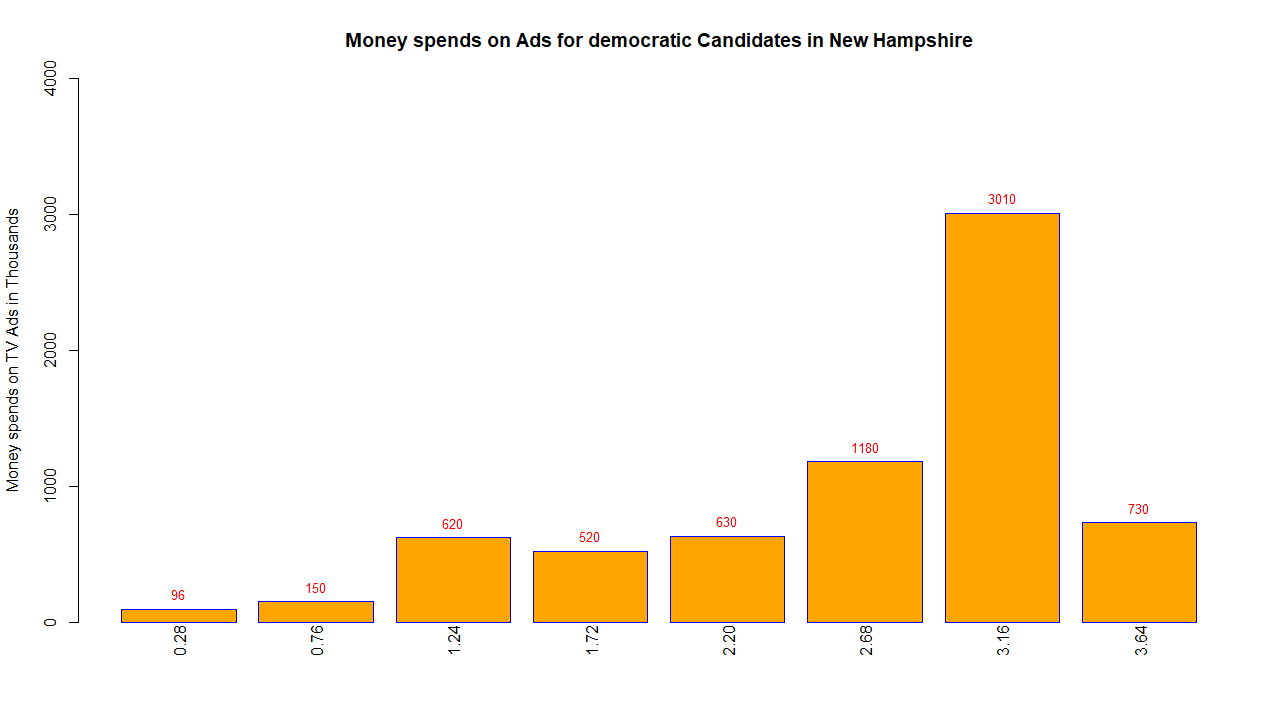
\includegraphics[width=0.9\textwidth]{figures/Newhampshire.png}
    \caption{Money spending on Ads in New Hampshire}
    \label{Newhampshire}
\end{figure}

\begin{figure}[H]
    \centering
    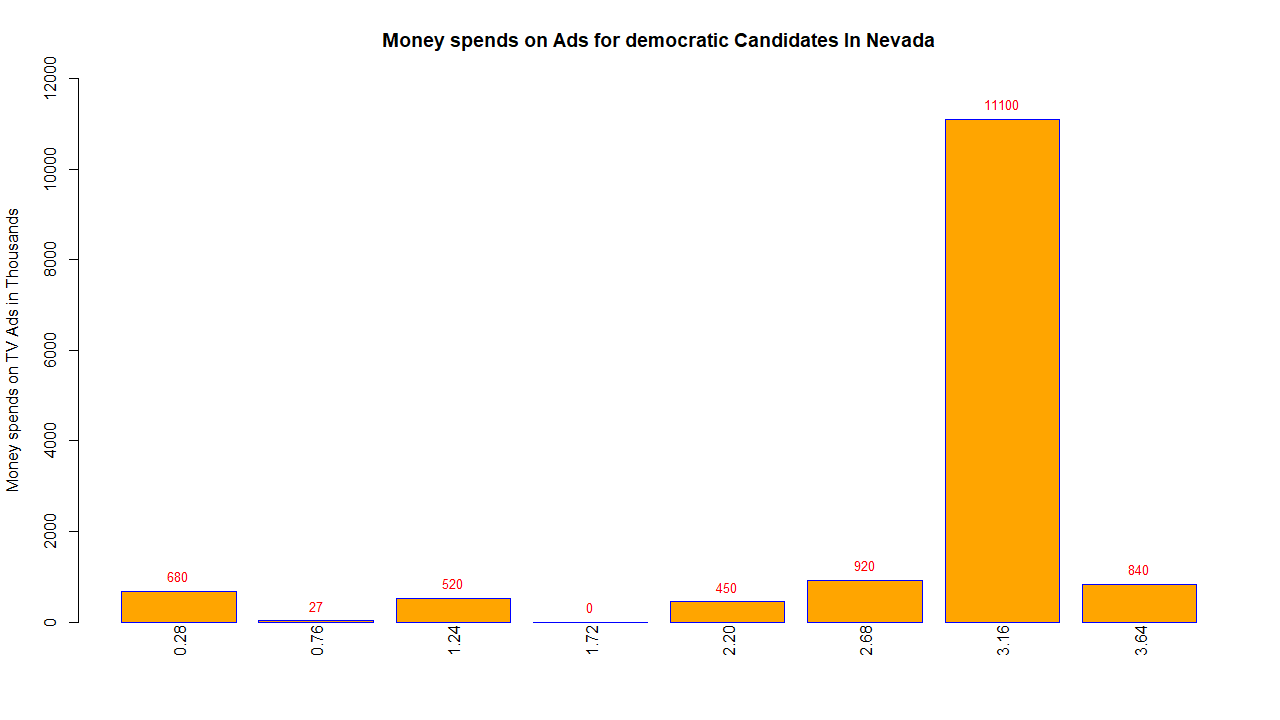
\includegraphics[width=0.9\textwidth]{figures/Nevada.png}
    \caption{Money spending on Ads in Nevada}
    \label{Nevada}
\end{figure}

\subsection{Funding}
Figures \ref{Total} to \ref{Others} shows funding from small and big donors,  self funding and funding from other sources.  
\begin{figure}[H]
    \centering
    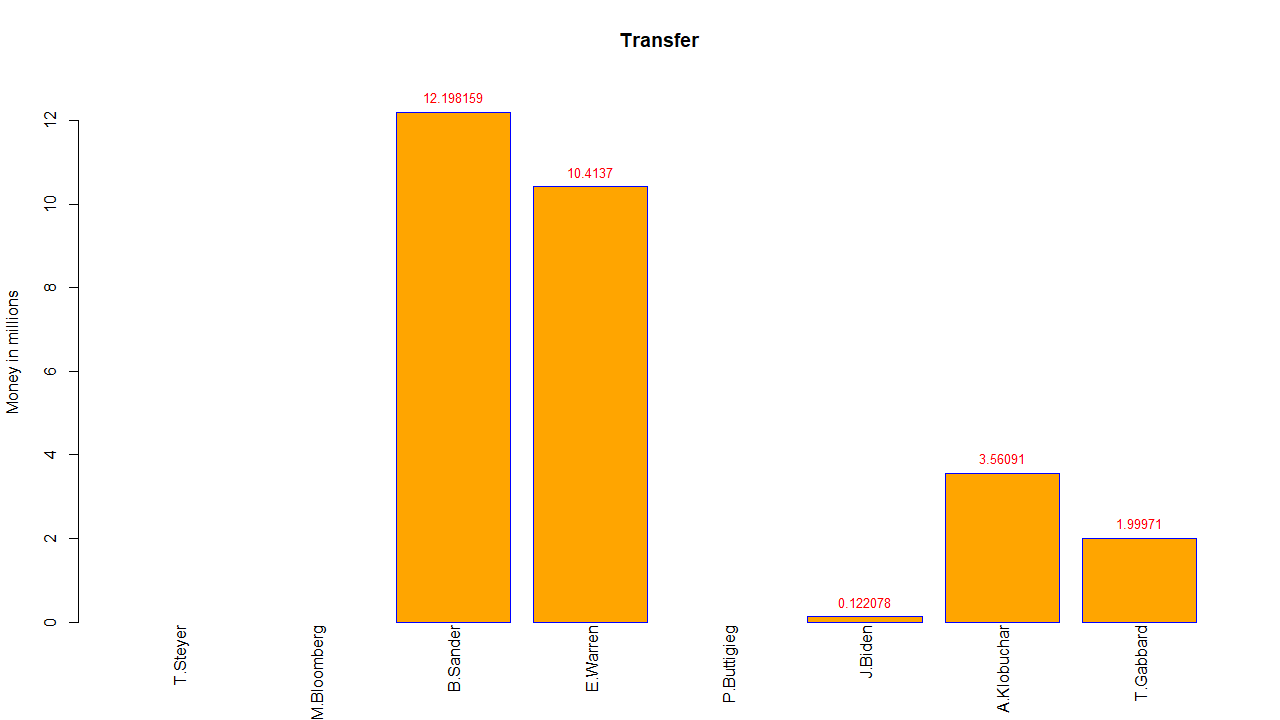
\includegraphics[width=0.9\textwidth]{figures/Total.png}
    \caption{Total Funding}
    \label{Total}
\end{figure}

\begin{figure}[H]
    \centering
    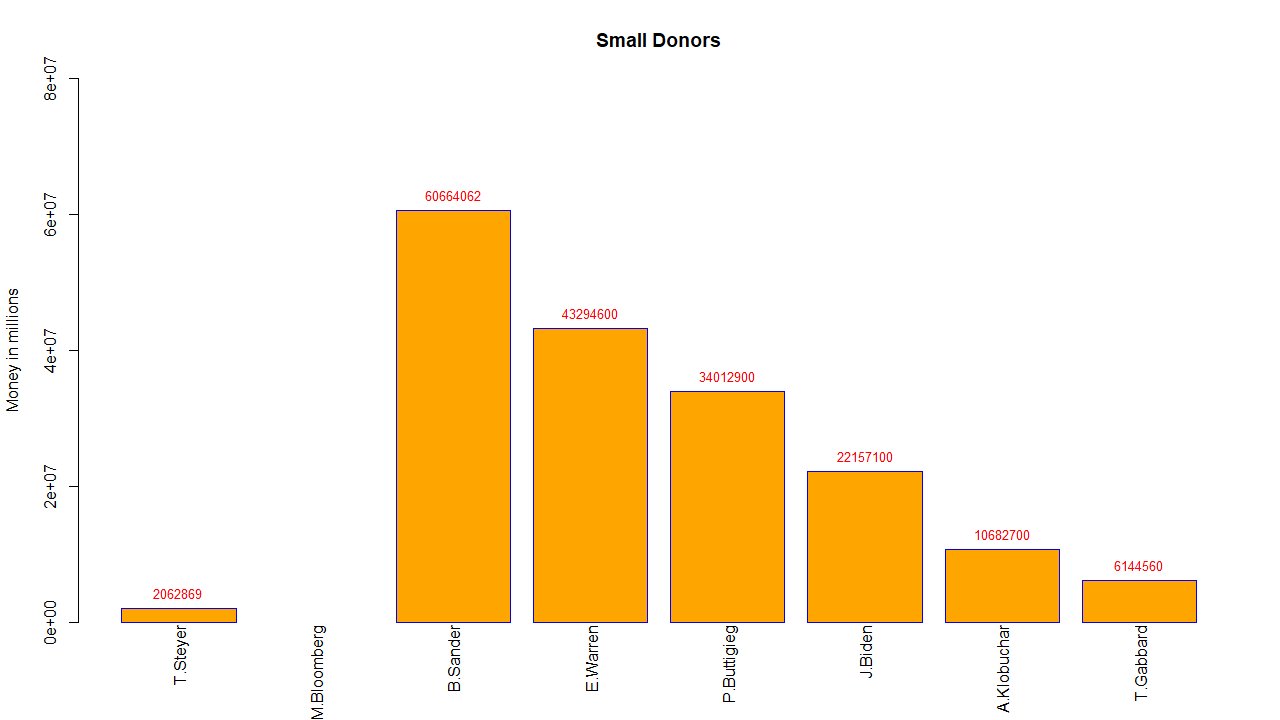
\includegraphics[width=0.9\textwidth]{figures/Small Donors.png}
    \caption{Small Donors Funding}
    \label{Small Donors}
\end{figure}

\begin{figure}[H]
    \centering
    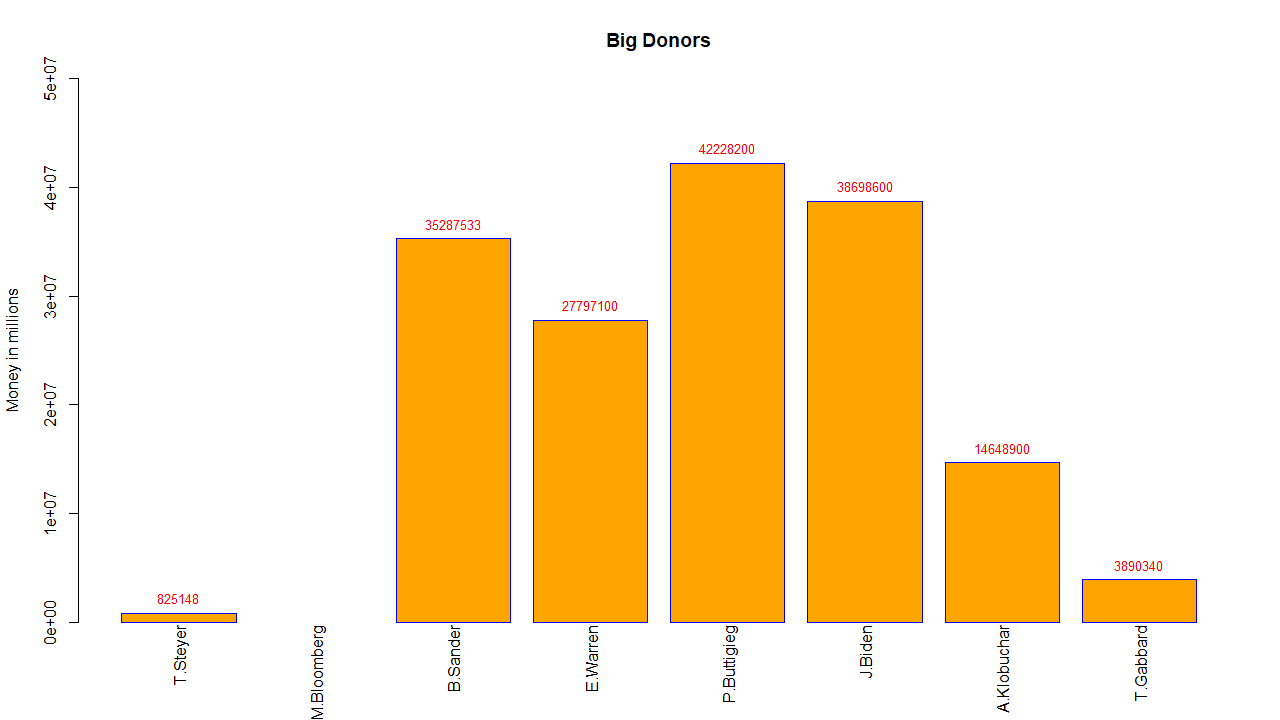
\includegraphics[width=0.9\textwidth]{figures/Bigdonor.png}
    \caption{Big donors Funding}
    \label{Bigdonor}
\end{figure}

\begin{figure}[H]
    \centering
    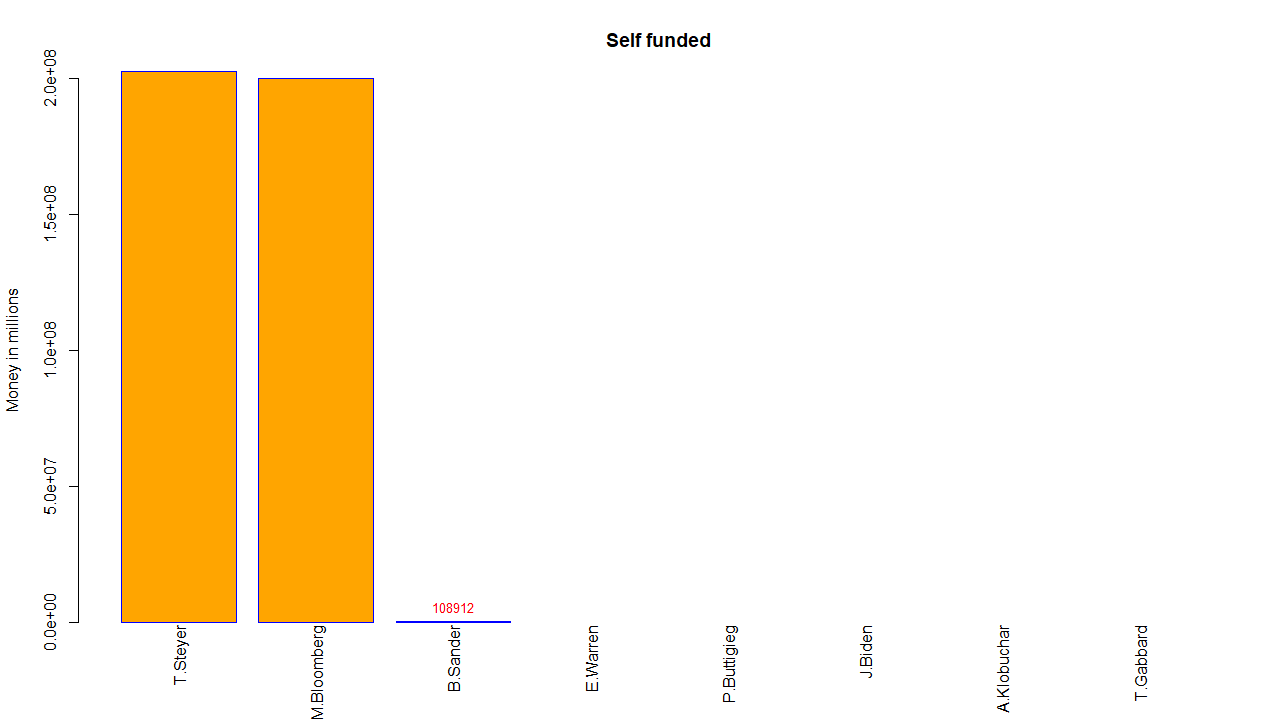
\includegraphics[width=0.9\textwidth]{figures/Selffunnded.png}
    \caption{Self funnded Funding}
    \label{Selffunnded}
\end{figure}

\begin{figure}[H]
    \centering
    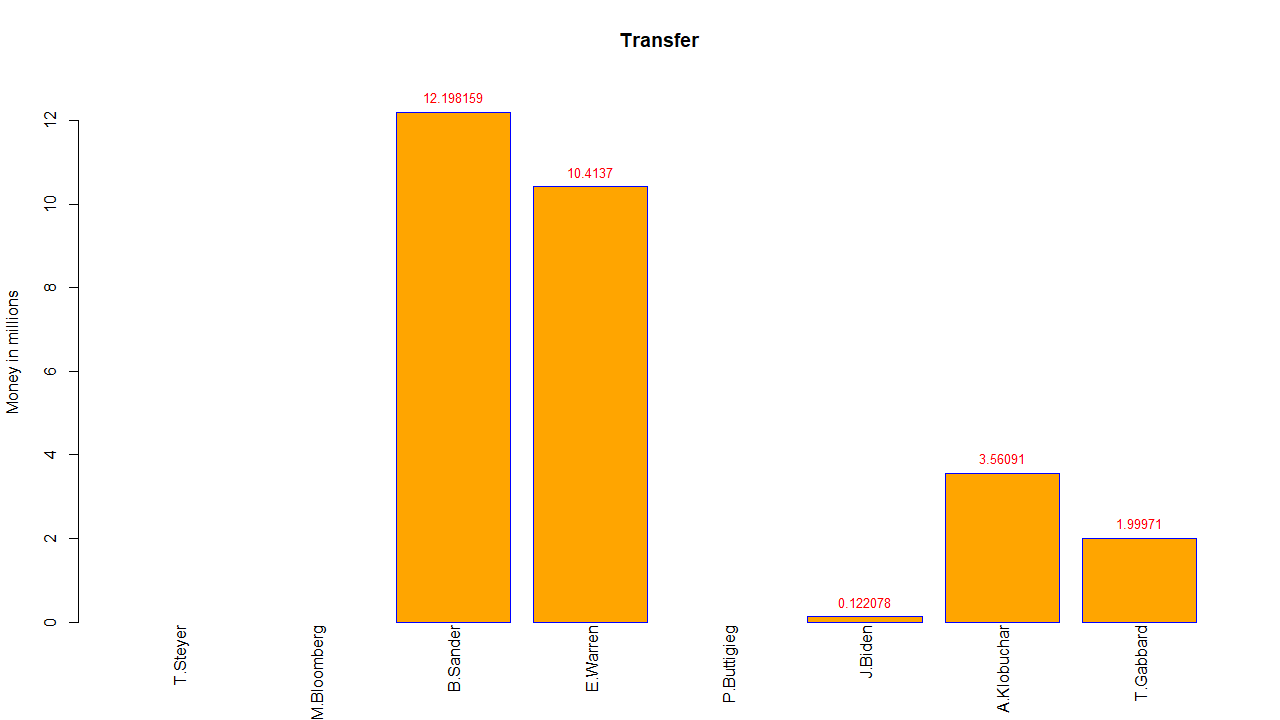
\includegraphics[width=0.9\textwidth]{figures/Transfer.png}
    \caption{Transfer Funding}
    \label{Transfer}
\end{figure}

\begin{figure}[H]
    \centering
    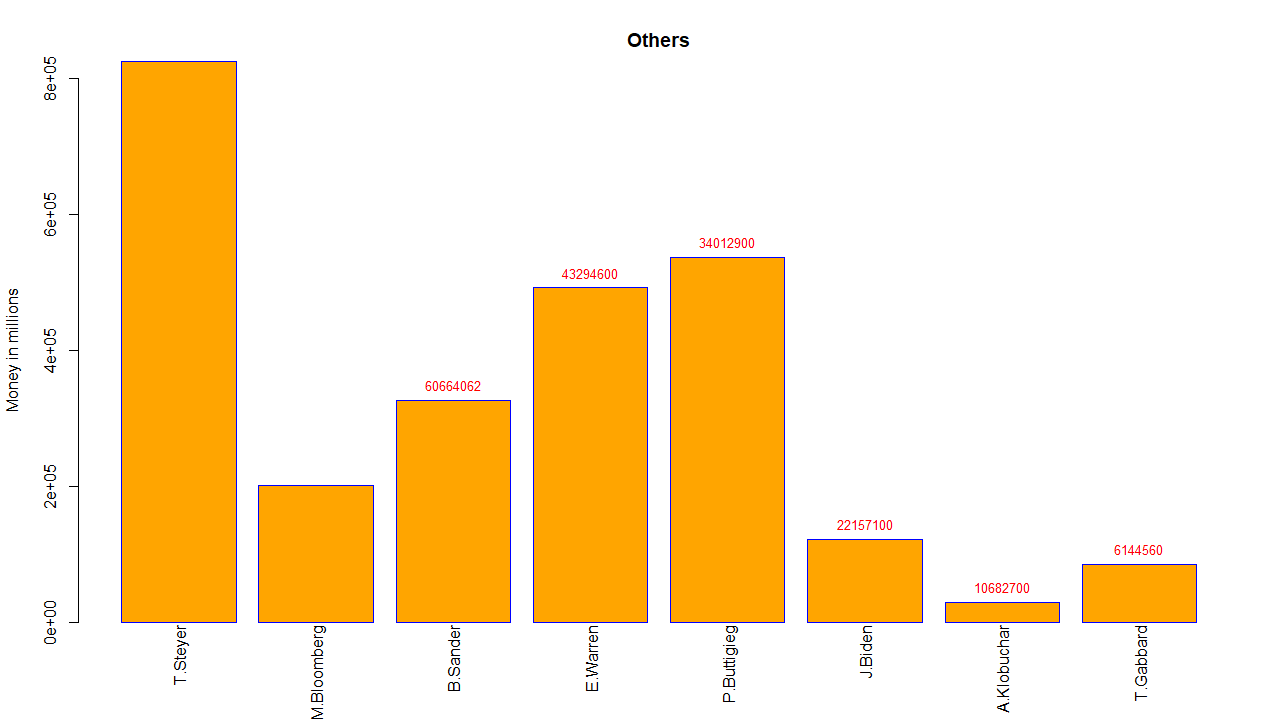
\includegraphics[width=0.9\textwidth]{figures/Others.png}
    \caption{Others Sources Funding}
    \label{Others}
\end{figure}
